% Generated from the public primitive catalog. Original Atlas drawing; Apache-2.0.
% Target: sm3-256; view: detail
\documentclass[border=9pt]{standalone}
% Original Atlas figure theme. Apache-2.0; see the repository LICENSE.
\usepackage[T1]{fontenc}
\usepackage{lmodern}
\usepackage{amsmath,amssymb}
\usepackage{tikz}
\usetikzlibrary{arrows.meta,positioning,calc,fit,backgrounds,decorations.pathreplacing,matrix}
\definecolor{atlasInk}{HTML}{172235}
\definecolor{atlasTeal}{HTML}{0D7B7D}
\definecolor{atlasMuted}{HTML}{637278}
\definecolor{atlasFill}{HTML}{EAF4F2}
\definecolor{atlasLine}{HTML}{B6C8C7}
\tikzset{
  every picture/.style={line width=.65pt,draw=atlasInk,>=Latex},
  every node/.style={text=atlasInk,font=\sffamily\small},
  box/.style={draw,rounded corners=1.5pt,minimum height=.9cm,minimum width=1.6cm,align=center,inner sep=6pt,fill=white},
  accent/.style={box,draw=atlasTeal,fill=atlasFill},
  wire/.style={->,line width=.7pt},
  keywire/.style={wire,draw=atlasTeal,dashed},
  xor/.style={draw,circle,fill=white,inner sep=0pt,minimum size=.38cm},
  add/.style={draw,rectangle,fill=white,inner sep=0pt,minimum size=.38cm},
  note/.style={font=\sffamily\scriptsize,text=atlasMuted,align=center},
  phase/.style={font=\sffamily\small\bfseries,text=atlasTeal},
  group/.style={draw=atlasLine,dashed,rounded corners=2pt,inner sep=8pt}
}
\newcommand{\rotl}{\mathbin{\lll}}
\newcommand{\rotr}{\mathbin{\ggg}}
\newcommand{\kx}{\operatorname{Keccak}\!\text{-}\!f[1600]}

\newcommand{\AtlasKeyBits}{k}
\newcommand{\AtlasKeyWords}{N_k}
\newcommand{\AtlasRounds}{N_r}
\newcommand{\AtlasPriorRounds}{N_r-1}
\newcommand{\AtlasRoundKeys}{N_r+1}
\newcommand{\AtlasDoubleRounds}{N_r/2}
\newcommand{\AtlasSixRoundGroups}{N_r/6}
\newcommand{\AtlasFLGroups}{N_r/6-1}
\newcommand{\AtlasRoundStart}{24-n}
\newcommand{\AtlasBlockBits}{512}
\newcommand{\AtlasOutputBits}{256}
\newcommand{\AtlasStateBits}{256}
\newcommand{\AtlasNonceBits}{v}
\newcommand{\AtlasCounterBits}{q}
\newcommand{\AtlasStreamBlockBits}{b}
\newcommand{\AtlasRate}{r}
\newcommand{\AtlasCapacity}{c}
\newcommand{\AtlasSteps}{64}
\newcommand{\AtlasLastStep}{63}
\newcommand{\AtlasWordBits}{32}
\newcommand{\AtlasHashWords}{8}
\newcommand{\AtlasFeedForward}{\oplus}
\newcommand{\AtlasByteOrder}{big-endian}
\newcommand{\AtlasDomain}{01}
\newif\ifAtlasXof
\AtlasXoffalse
\begin{document}
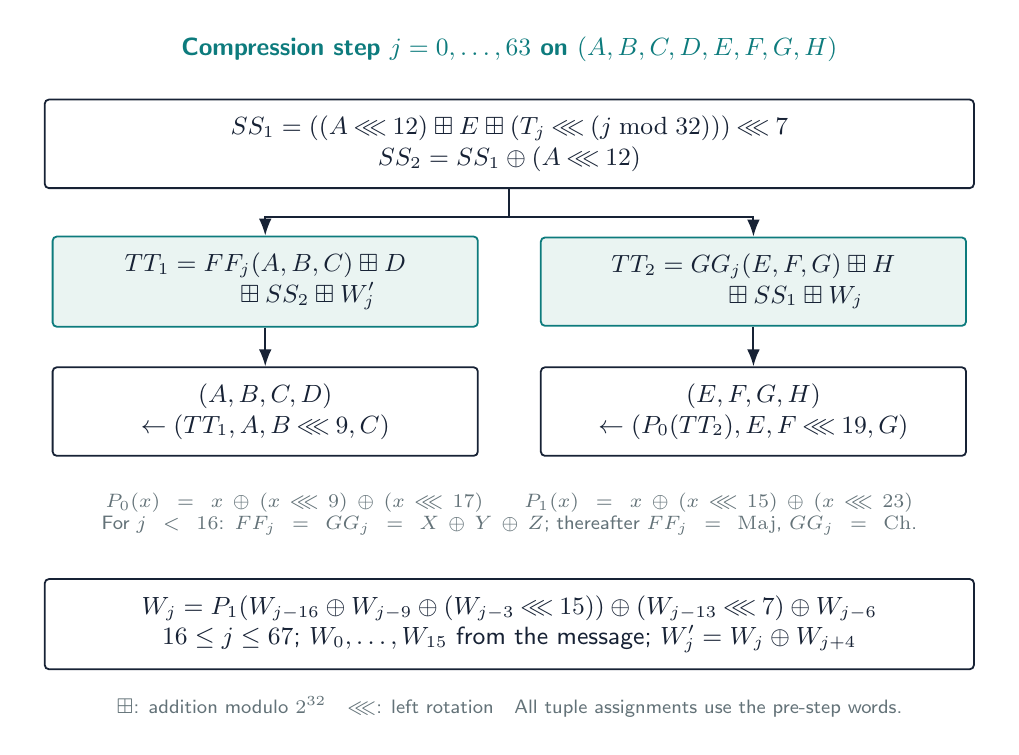
\begin{tikzpicture}
  \node[phase] at (6,4.1) {Compression step $j=0,\ldots,\AtlasLastStep$ on $(A,B,C,D,E,F,G,H)$};
  \node[box,minimum width=11.8cm] (ss) at (6,2.9) {$SS_1=((A\rotl12)\boxplus E\boxplus(T_j\rotl(j\bmod32)))\rotl7$\\$SS_2=SS_1\oplus(A\rotl12)$};
  \node[accent,minimum width=5.4cm] (left) at (2.9,1.15) {$TT_1=FF_j(A,B,C)\boxplus D$\\$\phantom{TT_1={}}\boxplus SS_2\boxplus W'_j$};
  \node[accent,minimum width=5.4cm] (right) at (9.1,1.15) {$TT_2=GG_j(E,F,G)\boxplus H$\\$\phantom{TT_2={}}\boxplus SS_1\boxplus W_j$};
  \draw[wire] (ss.south) -- ++(0,-.35) -| (left.north);
  \draw[wire] (ss.south) -- ++(0,-.35) -| (right.north);
  \node[box,minimum width=5.4cm] (lu) at (2.9,-.5) {$(A,B,C,D)$\\$\gets(TT_1,A,B\rotl9,C)$};
  \node[box,minimum width=5.4cm] (ru) at (9.1,-.5) {$(E,F,G,H)$\\$\gets(P_0(TT_2),E,F\rotl19,G)$};
  \draw[wire] (left) -- (lu); \draw[wire] (right) -- (ru);
  \node[note,text width=12cm] at (6,-1.8) {$P_0(x)=x\oplus(x\rotl9)\oplus(x\rotl17)$\qquad $P_1(x)=x\oplus(x\rotl15)\oplus(x\rotl23)$\\For $j<16$: $FF_j=GG_j=X\oplus Y\oplus Z$; thereafter $FF_j=\mathrm{Maj}$, $GG_j=\mathrm{Ch}$.};
  \node[box,minimum width=11.8cm] at (6,-3.2) {$W_j=P_1(W_{j-16}\oplus W_{j-9}\oplus(W_{j-3}\rotl15))\oplus(W_{j-13}\rotl7)\oplus W_{j-6}$\\$16\le j\le67$; $W_0,\ldots,W_{15}$ from the message; $W'_j=W_j\oplus W_{j+4}$};
  \node[note] at (6,-4.25) {$\boxplus$: addition modulo $2^{32}$\quad $\rotl$: left rotation\quad All tuple assignments use the pre-step words.};
\end{tikzpicture}

\end{document}
